% Content for the test report for LSP-00-00

The tests were performed primarily from an Apple laptop computer running OS X 10.11.6, wirelessly connected to the Internet and using the NCSA VPN at \texttt{vpn.ncsa.illinois.edu}.
API Aspect queries were performed using a combination of the Python \texttt{requests} package and the \texttt{curl} command.
Notebooks were executed using Jupyter versions up through 5.4.1 and Python version 3.6.1.
The Portal was accessed using Safari 11.0.2.

\subsection{API Aspect tests}

The API Aspect tests made use of the "v0" \texttt{dbserv} service at 

\begin{center}
\texttt{http://lsst-qserv-dax01.ncsa.illinois.edu:5000/db/v0/tap/sync}.
\end{center}

This service accepts SQL queries, forwards them to Qserv for execution, and returns the results as JSON structures.
The open-source Python \emph{Requests} package\footnote{\texttt{http://github.com/requests/requests}} was used to perform the HTTP GET and POST operations required, and to parse the returned JSON structures into Python dictionaries.

\subsubsection{Table presence verification}
\label{sect:lsp-00-00-api-tables}

API Aspect \verb|dbserv| queries (\texttt{SHOW DATABASES} and \texttt{SHOW TABLES}) were used to establish the set of databases available, and within those databases, identify the WISE catalog tables of interest for the tests.

\begin{table}[h]
\centering
\begin{tabular}{p{0.4\textwidth} l l}
WISE catalog & PDAC database & PDAC table \\ \hline
AllWISE Source Catalog & \verb|wise_00| & \verb|allwise_p3as_psd| \\
AllWISE Multi-Epoch Photometry Table & \verb|wise_00| & \verb|allwise_p3as_mep| \\
All-Sky Single Exposure (L1b) Source Table & \verb|wise_4band_00| & \verb|allsky_4band_p1bs_psd| \\
3-Band Cryo Single Exposure (L1b) Source Table & \verb|wise_3band_00| & \verb|allsky_3band_p1bs_psd| \\
Post-Cryo Single Exposure (L1b) Source Table & \verb|wise_2band_00| & \verb|allsky_2band_p1bs_psd| \\
NEOWISE-R Year 1 Single Exposure Source Table & \verb|neowiser_yr1_00| & \verb|neowiser_yr1_p1bs_psd| \\
\end{tabular}
\caption{WISE tables as discovered through the PDAC DAX service}
\label{tab:wisetables}
\end{table}

\subsubsection{Table Schemas}
\label{sect:lsp-00-00-api-schema}

Schemas for the tables were obtained from \verb|DESCRIBE| queries on \verb|dbserv|.
The schemas were compared programmatically against those obtained from the 
appropriate IRSA program interface:

\begin{center}
\verb|https://irsa.ipac.caltech.edu/cgi-bin/Gator/nph-dd?mode=xml&catalog=|\textit{table}.
\end{center}

The results were parsed with the Python standard library class \verb|xml.etree.ElementTree|.
Comparison of the schemas was carried out in Python, without regard to the ordering of columns.
The following discrepancies were observed (details are preserved in the test notebook):

\begin{itemize}
\item The \verb|dec| column in each table was renamed to \verb|decl| to avoid a conflict with a reserved word in the Qserv implementation database.
\item The Qserv implementation adds special columns \verb|chunkId| and \verb|subChunkId| to each partitioned table.
\item The original column names in the \verb|wise_2band_00.allsky_2band_p1bs_psd| table all appear in the PDAC version converted to uppercase.
\item For some tables, The IRSA-published schemas via the program interface have additional columns compared to what is displayed in the IRSA Gator UI and, apparently, in addition to what was included in the export files used to load the PDAC Qserv.  
This was assessed to be irrelevant to the objectives of this test, and no serious effort was made to determine the reasons in time for this report, as this would have required IRSA staff time that was in short supply.
IRSA support tickets will be filed to ensure that the discrepancies are ultimately understood and, if possible and desirable, corrected.
The affected tables are:
  \begin{itemize}
  \item \verb|allwise_p3as_psd|: 36 columns appear in the IRSA program interface schema that do not appear in the PDAC table.
    Most of these are associated with a proper motion model fit.
  \item \verb|allsky_4band_p1bs_psd|: 20 columns appear in the IRSA program interface schema that do not appear in the PDAC table.
    16 of these seem to be intermediate data products of the photometry pipeline, including zero-point corrected PSF and aperture magnitudes and the zero points themselves.
  \item \verb|neowiser_yr1_p1bs_psd| (compared against the IRSA program interface for the ``live'' table \verb|neowiser_p1bs_psd|): 24 columns appear in the IRSA program interface schema that do not appear in the PDAC table.  
    These again appear to be a set of intermediate data products.
  \end{itemize}
\end{itemize}

\subsubsection{Row counts}
\label{sect:lsp-00-00-api-count}

Row counts were obtained from \verb|COUNT(*)| queries against all six tables.
These queries require accessing all chunks and subchunks in the Qserv partitioning and therefore resulted in table scans taking several minutes of wall clock time each.
The row counts and representative query durations are shown in Table \ref{tab:wisetablerows}.
The pattern of query times has not been fully understood; \verb|allwise_p3as_psd| is a notable outlier.
The row counts were compared to those advertised in the WISE documentation at IRSA.
They agree exactly except for the AllWISE Multi-Epoch Photometry Table, \verb|allwise_p3as_mep|, for which 42,759,337,365 rows are reported in the IRSA documentation, a difference of 761,630,509 or 1.8\%.
This discrepancy has not yet been understood.

\begin{table}[h]
\centering
\begin{tabular}{l r r}
PDAC WISE table & Rows & \texttt{COUNT(*) duration} \\ \hline
\verb|allwise_p3as_psd| & 747,634,026 & 798s \\
\verb|allwise_p3as_mep| & 41,997,706,856 & 1457s \\
\verb|allsky_4band_p1bs_psd| & 9,479,433,101 & 993s \\
\verb|allsky_3band_p1bs_psd| & 3,703,319,374 & 278s \\
\verb|allsky_2band_p1bs_psd| & 7,337,642,955 & 535s \\
\verb|neowiser_yr1_p1bs_psd| & 18,468,575,586 & 759s \\
\end{tabular}
\caption{Row counts in PDAC WISE tables, with durations of the associated \texttt{COUNT(*)} queries}
\label{tab:wisetablerows}
\end{table}

\subsection{Portal Aspect}
\label{sect:lsp-00-00-portal}

The Portal Aspect was accessed in order to verify the accessibility of the WISE catalog data.

This work covers step 6 of the LSP-00-00 test case procedure.

\subsubsection{Step 6a}

The front page of the Portal Aspect for this test was:

\begin{center}
\texttt{https://lsst-sui-proxy01.ncsa.illinois.edu/suit/}
\end{center}

\subsubsection{Step 6b}

The front page presents an ``LSST Data'' screen which offers the catalog data available for access, associated with three ``projects'': SDSS, AllWISE, and the WISE and NEOWISE single-epoch photometry.

The radio buttons under the project selector show the tables available for selection.
All six WISE tables covered by this test specification are available, as seen in the following screen shots.

\begin{figure}
  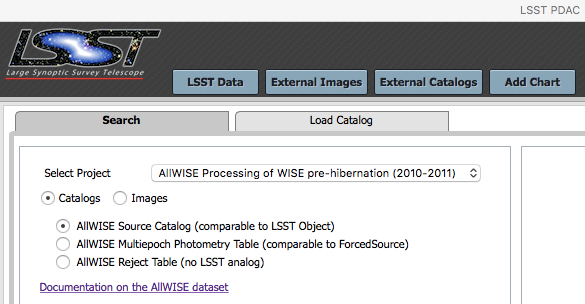
\includegraphics[width=\linewidth]{lsp-00-00/AllWISE-table-selection.png}
  \caption{AllWISE tables available for query in the Portal}
  \label{fig:portal-allwise-sel}
\end{figure}

\begin{figure}
  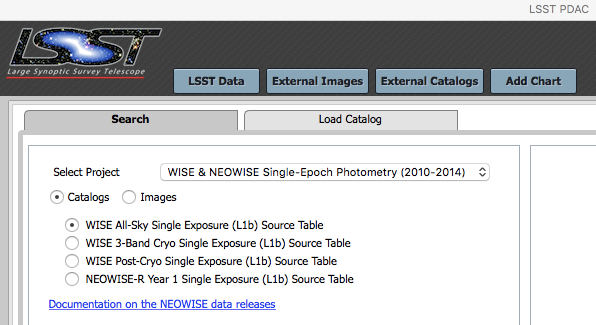
\includegraphics[width=\linewidth]{lsp-00-00/Single-Epoch-table-selection.png}
  \caption{WISE and NEOWISE single-epoch photometry tables available for query in the Portal}
  \label{fig:portal-singleepoch-sel}
\end{figure}

Given a selected table, the UI presents a selector for the type of search to be performed, offering a variety of options for spatial region searches including cone, ellipse, box, and polygon, as well as a multi-object cone search and a free-form all-sky search.
This UI element is shown in Figure \ref{fig:portal-search-methods} below.

\begin{figure}
  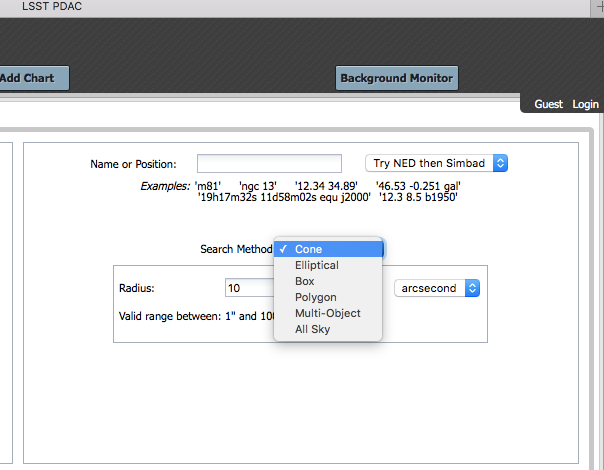
\includegraphics[width=\linewidth]{lsp-00-00/search-methods-pane.png}
  \caption{Search methods available for Portal queries on the WISE tables}
  \label{fig:portal-search-methods}
\end{figure}

\subsubsection{Step 6c}

The Portal also provides a UI element, shown in Figure \ref{fig:portal-schema-browser} displaying the entire table schema in a scrolling region, with, among other features, the ability to apply restrictions to any column for application in the query to be performed.
It was not a goal of this test to specifically validate the correct display of the schema, but some spot checks were performed and the results were as expected.
For instance, the schema display was observed to follow the expected pattern of whether W3- and W4-related were available in the selected table(s).
(The nature of the scrolling region provided for this selector inhibits easy capture of the entire content.
It would be useful for the final Portal to provide a UI element facilitating download of the entire schema.)
The schema anomalies reported in section \ref{sect:lsp-00-00-api-schema} above were also observed here, e.g., the uppercase conversion of the original column names in the \verb|allsky_2band_p1bs_psd| column.

Note that units and descriptions are not provided in the UI, though the layout anticipates them;
this is a consequence of the absence of a full \verb|metaserv| implementation at the time of the tests.

\begin{figure}
  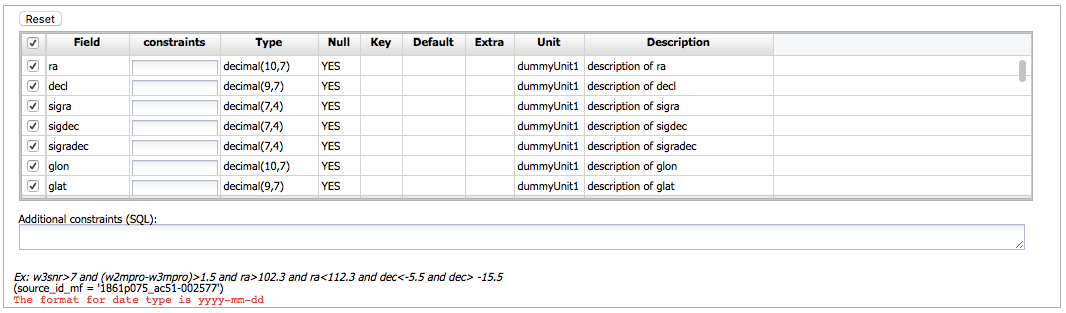
\includegraphics[width=\linewidth]{lsp-00-00/schema-browser.png}
  \caption{Schema browser and column-restriction API in the Portal, for WISE 3-band table}
  \label{fig:portal-schema-browser}
\end{figure}

The test specification calls for doing spot queries around (ra=0, dec=0); 
it turns out to be more useful to do them away from ra=0 so that in the default plots in the Portal plotting tool the points are not split across values just below 360 and just above 0.
(The values can be rescaled to (-180,180), of course, but this requires an extra step.)

100-arcsecond cone searches were successfully performed at (ra=1, dec=0) for all six tables.
The \verb|allsky_3band_p1bs_psd| search returned no rows, corresponding to this sky location not being included in the brief period of 3-band observation.
Screen shots are provided for \verb|allwise_p3as_psd| and \verb|neowiser_yr1_p1bs_psd|, and tabular results for all five non-empty queries are stored in the DMTR-52 repository.
Note the much larger number of sources for the NEOWISE-R single-epoch table query.

\begin{figure}
  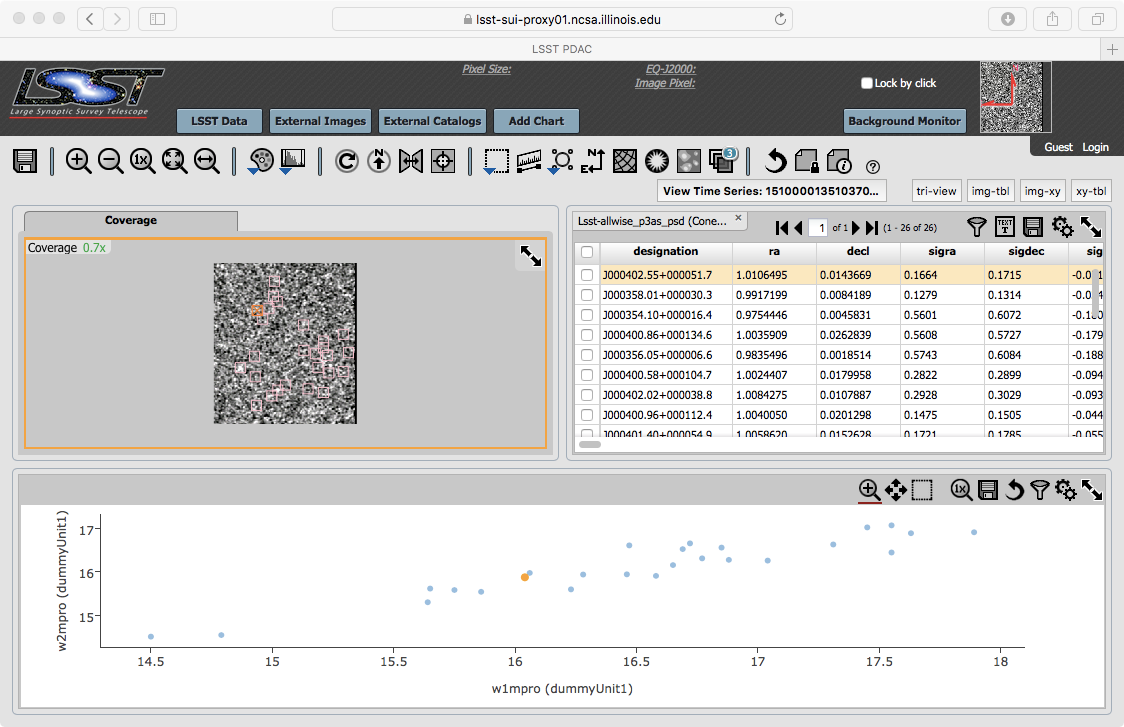
\includegraphics[width=\linewidth]{lsp-00-00/Portal-allwise_p3as_psd.png}
  \caption{Query at ra=1, dec=0 on the AllWISE Source Catalog}
  \label{fig:portal-query-allwise-psd}
\end{figure}

\begin{figure}
  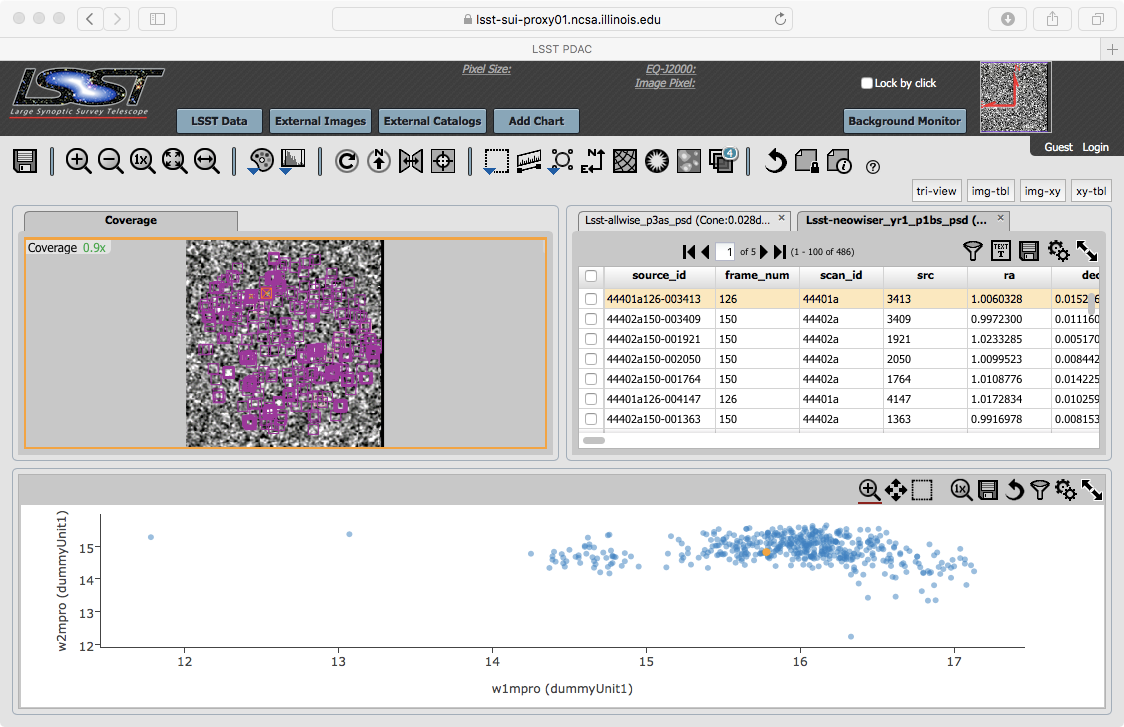
\includegraphics[width=\linewidth]{lsp-00-00/Portal-neowiser_yr1_p1bs_psd.png}
  \caption{Query at ra=1, dec=0 on the NEOWISE-R Year 1 Single-Epoch Source Catalog}
  \label{fig:portal-query-neowiser-psd}
\end{figure}
